\documentclass{beamer}

\usepackage[utf8]{inputenc}
\usepackage[english]{babel}

\usepackage{graphicx}
\usepackage{amsmath}
\usepackage{amssymb}
\usepackage{amsthm}
\usepackage{array}

\usepackage{alltt}

\addtocounter{footnote}{1}
\setcounter{tocdepth}{5}
\setcounter{secnumdepth}{5}
\renewcommand{\floatpagefraction}{0.75}

%Information to be included in the title page:
\title{Using textures with OpenGL 3.3}
\author{Alexander Christensen}
\institute{Department of Computer Science \\ University of Copenhagen}
\date{2019}

%% Reference an equation, a figure, or a section

%% \secref{label} - make a reference to a section
\newcommand{\secref}[1]{Section~\ref{#1}}

%% \eqref{reference} - make a reference to an equation
%%\newcommand{\eqref}[1]{(\ref{#1})}

%% \figref{reference} - make a reference to an figure
\newcommand{\figref}[1]{Figure~\ref{#1}}

\newcommand{\basetop}[1]{\vtop{\vskip-1ex\hbox{#1}}}
\newcommand{\source}[1]{\let\thefootnote\relax\footnotetext{\scriptsize\textcolor{kugray1}{Source: #1}}}

%\bibliographystyle{longalpha}
%\bibliography{refs}

%% -*- Mode: latex -*-

%% Macros defined during a long time and used much
% plus - a plus sign
\newcommand{\plus}{+}

% minus - a minus having the same width as a plus
\newlength{\minuswidth}
\settowidth{\minuswidth}{+}
\newlength{\minusheight}
\settoheight{\minusheight}{+}
\newcommand{\minus}{\rule[0.5\minusheight]{\minuswidth}{0.5pt}}

% The basis vector standard
%\renewcommand{\vec}[1]{\boldsymbol{#1}}
\newcommand{\grad}{\operatorname{\nabla}}
\newcommand{\curl}{\operatorname{\text{curl}}}
\newcommand{\divergence}{\operatorname{\text{div}}}
\newcommand{\vecop}{\operatorname{\text{vec}}}
\newcommand{\diag}{\operatorname{\text{diag}}}
\renewcommand{\Re}{\mathbb{R}}
\newcommand{\Co}{\mathbb{C}}
\newcommand{\In}{\mathbb{Z}}
\newcommand{\sign}{\operatorname{sgn}}
%\newcommand{\trace}{\operatorname{Tr}}
\newcommand{\arctantwo}{\ensuremath{\arctan\!2}}
%\newcommand{\mat}[1]{\ensuremath{\boldsymbol{#1} }}
\newcommand{\I}{\mat{1}}
\newcommand{\crossmat}[1]{\ensuremath{\boldsymbol{#1}^{\times} }}
\newcommand{\jacobian}[1]{\ensuremath{\boldsymbol{\mathit{#1}} }}
\newcommand{\set}[1]{\ensuremath{ \boldsymbol{#1} }}
\newcommand{\func}[1]{{\bf{#1}}}
\newcommand{\enorm}[1]{\ensuremath{\left\| #1 \right\|_{_2}}}
%\newcommand{\norm}[1]{\ensuremath{\left\| #1 \right\|}}
\newcommand{\bdet}[1]{\ensuremath{\left| #1 \right|}}
\newcommand{\abs}[1]{\ensuremath{\left| #1 \right|}}
\newcommand{\rtm}{$^{\textrm{®}}$}


\newcommand{\kenny}[1]{ #1 }
\newcommand{\henrik}[1]{ #1 }


%% \maya - the maya signature
\newcommand{\maya}{$ \texttt{Maya}^{\text{\texttrademark}} $}

%% \fat{symbol} - make this symbol fat
\newcommand{\fat}[1]{\mathit{\mathbf{#1}}}
%% \newcommand{\fat}[1]{\hbox{\boldmath $ #1 $}}

%% \vec{symbol} - Vector
%% \renewcommand{\vec}[1]{\mathbf{#1}}
\renewcommand{\vec}[1]{\fat{#1}}

%% \mat{symbol} - Matrix
%%\newcommand{\mat}[1]{\ensuremath{\boldsymbol{#1} }}
\newcommand{\mat}[1]{\fat{#1}}

%% \ezero,...,\ethree - the spin matrices
\newcommand{\ezero}{\begin{bmatrix} 1 & 0 \\  0 &  1 \end{bmatrix}}
\newcommand{\eone}{\begin{bmatrix} i & 0 \\  0 & -i \end{bmatrix}}
\newcommand{\etwo}{\begin{bmatrix} 0 & 1 \\ -1 &  0 \end{bmatrix}}
\newcommand{\ethree}{\begin{bmatrix} 0 & i \\  i &  0 \end{bmatrix}}

%% \quat{symbol} - Quaternion
%% \newcommand{\quat}[1]{\mathbf{#1}}
\newcommand{\quat}[1]{\fat{#1}}

%% \real{quaternion} - the real (scalar) part of a quaternion
\newcommand{\real}{\operatorname{real}}

%% \pure{quaternion} - the pure (vector) part of a quaternion
\newcommand{\pure}{\operatorname{pure}}

%% \sgn{symbol} - the sign of a symbol
\newcommand{\sgn}{\operatorname{sgn}}

%% \norm{symbol} - Norm of a vector/quaternion
\newcommand{\norm}[1]{\parallel {#1} \parallel}

%% \trace{matrix}
\newcommand{\trace}[1]{\mathrm{trace}(#1)}

% This is for code-snippets in the text.
\usepackage{fancyvrb}   %% Try to comment this out if problems with pdflatex
\newcommand{\code}[1]%
%{ \VerbatimInput[frame=none,fontsize=\footnotesize,numbers=none,label=\texttt{#1}]{#1}  }
{ \VerbatimInput[frame=single,fontsize=\footnotesize,numbers=left,label=\texttt{#1}]{#1}  }


%\newcommand{\todo}[1]{ {\Bf Todo:} #1}
\newcommand{\todo}[1]{ }

%\newcommand{\longversion}[1]{ #1 }
\newcommand{\longversion}[1]{ }


\mode<presentation>
{
  \usetheme{Diku}
  \beamertemplatenavigationsymbolsempty
  \setbeamercovered{invisible}
%  \setbeamercovered{transparent=15}
}

%% Kennys pseudocode environment

\newenvironment{pseudocode}{
  \begin{center}
    \begin{minipage}[t]{0.8\columnwidth}
      \footnotesize
      \rule{\columnwidth}{1pt}
    }{
      \rule{\columnwidth}{1pt}
    \end{minipage}
  \end{center}
}

{
\AtBeginSection[wef]
{
\begin{frame}
\frametitle{Table of Contents}
\tableofcontents[currentsection]{1}
\end{frame}
}
}


\begin{document}

% Set background to front page
\usebackgroundtemplate{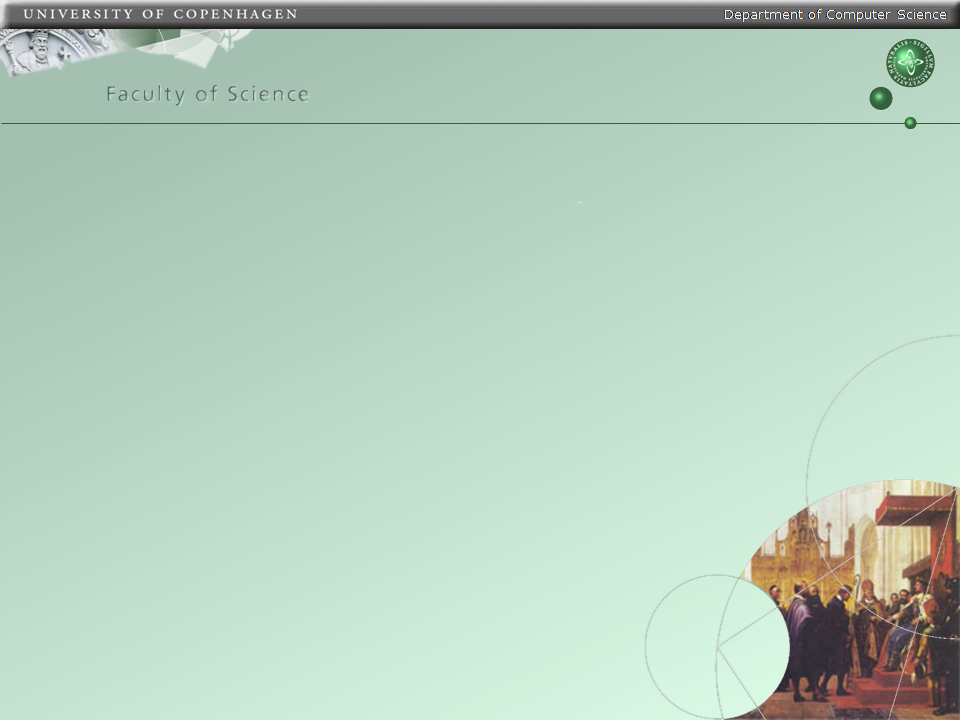
\includegraphics[width=\paperwidth,height=\paperheight]{front}}
{
\begin{frame}[plain]
  \titlepage
\end{frame}
}

% Set background to rest of pages
\usebackgroundtemplate{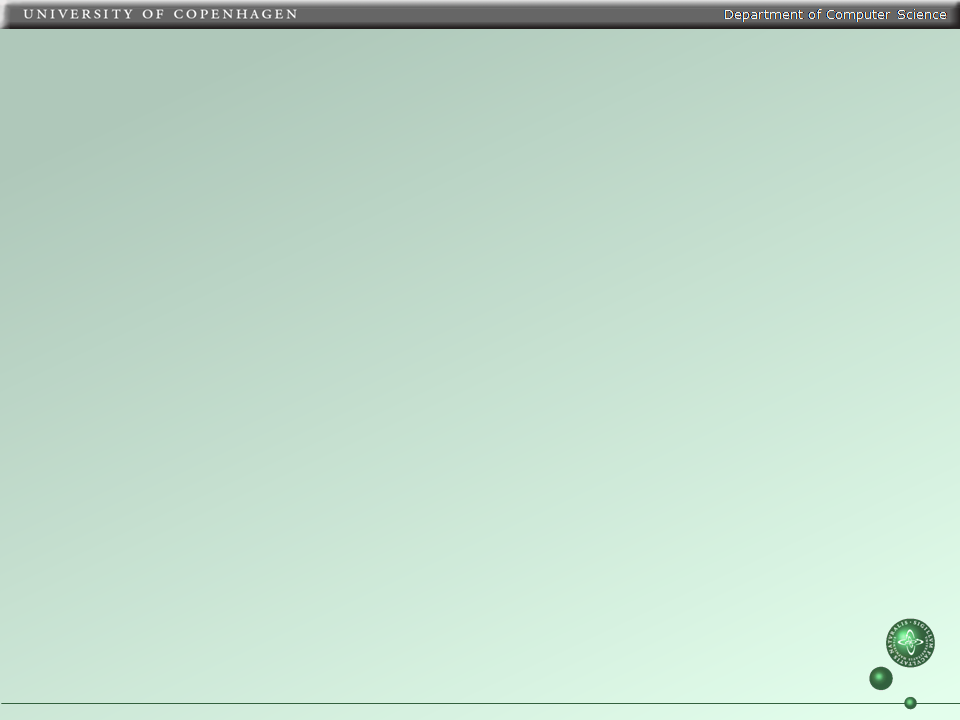
\includegraphics[width=\paperwidth,height=\paperheight]{background}}

%
%
%
\begin{frame}
\frametitle{Overview}
\tableofcontents
%% This is a text in first frame. This is a text in first frame. This is a text in first frame.
\end{frame}


%
%
%
\section{What is a texture?}
\begin{frame}
\frametitle{What is a Texture?}
A texture is an image that has been loaded to the GPU as a consecutive
block of memory.\\

OpenGL has no built-in functions for loading textures from the hard-disk.\\

Assume a 2D texture with four color channels (RGBA):

\begin{alltt}\footnotesize
int width, height;\\
GLubyte* ourTextureData = someFunctionToReadFromDisk("ourImage.png",\\
\ensuremath{\qquad}\&width, \&height);\\

GLuint ourTexture;\\
glGenTextures(1, ourTexture);\\
glBindTexture(GL\_TEXTURE\_2D, ourTexture);\\
glTexImage2D(GL\_TEXTURE\_2D, 0, GL\_RGBA, width, height, 0, GL\_RGBA,\\
\ensuremath{\qquad}GL\_UNSIGNED\_BYTE, ourTextureData);\\

\end{alltt}
\end{frame}


%
%
%
\section{Texture Coordinates}

\begin{frame}
\frametitle{Texture Coordinates}
We define a normalized coordinate system $T : \mathbb{R}^2$.
A coordinate in a texture is called a \textit{texel}, and is a discrete value.
To get a texel given real coordinates $(u,v)$ we can apply a filtering
function $f(u,v)\ :\ \mathbb{R}^2 \mapsto \mathbb{N}^2$.
\begin{figure}
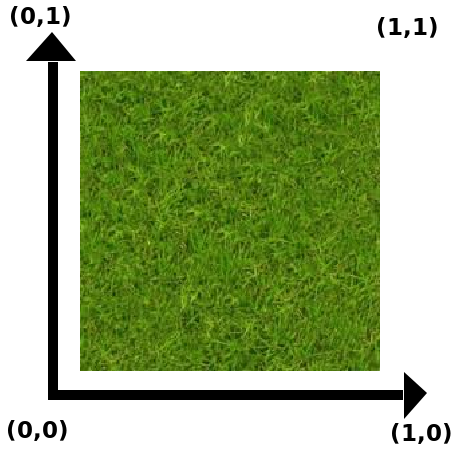
\includegraphics[width=0.5\textwidth]{images/textureCoordinates.png}
\end{figure}
\end{frame}


%
%
%
\begin{frame}
\frametitle{Texture Coordinates - Filtering}
\begin{figure}
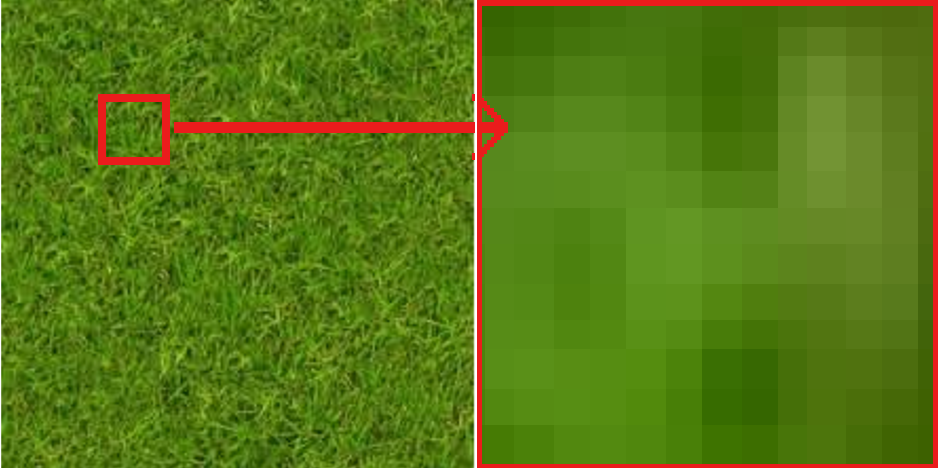
\includegraphics[width=0.7\textwidth]{images/filtering.png}
\end{figure}
Define a function for interpolating between texture coordinates:
\texttt{GL\_NEAREST :} choose nearest texel.\\
\texttt{GL\_LINEAR\ \  :} linearly interpolate over neibhbouring texels.
\end{frame}


%
%
%
\begin{frame}
\frametitle{Texture Coordinates - Clamping and Wrapping}
\begin{figure}
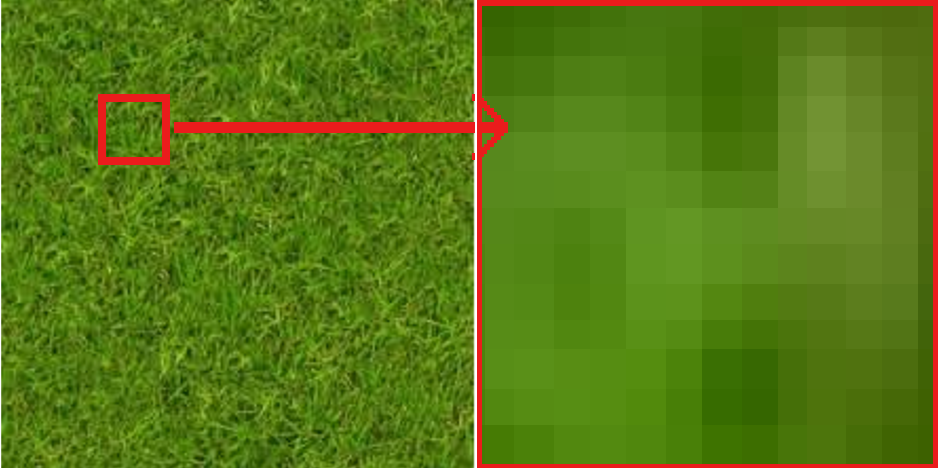
\includegraphics[width=0.7\textwidth]{images/filtering.png}
\end{figure}
Define a function for interpolating between texture coordinates:
\texttt{GL\_NEAREST :} choose nearest texel.\\
\texttt{GL\_LINEAR\ \  :} linearly interpolate over neibhbouring texels.
\end{frame}


%
%
%
\section{Texture Mapping}
\begin{frame}
Given a triangle with texture coordinates $(u1,v1)$, $(u2,v2)$, and $(u3,v3)$,
we wish to define a mapping, such that each vertex gets its own
texture coordinate.
\frametitle{Texture Mapping}
\begin{figure}
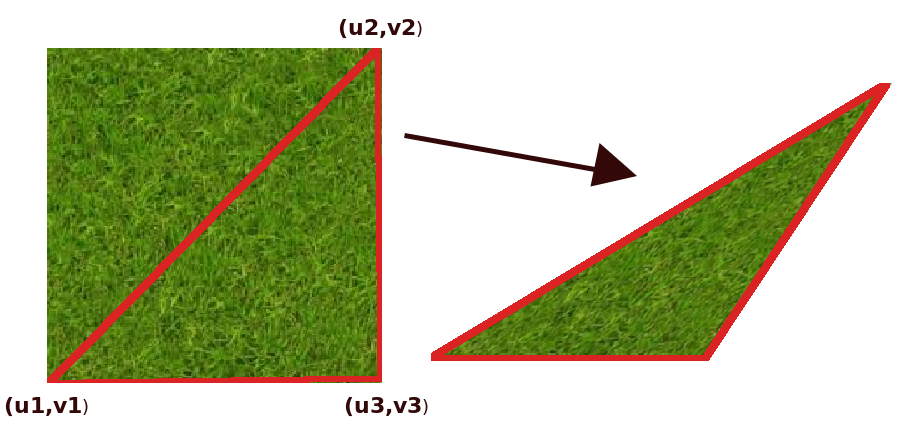
\includegraphics[width=0.9\textwidth]{images/textureMapping.png}
\end{figure}
\end{frame}


%
%
%
\begin{frame}
\frametitle{Texture Mapping - Vertex Shader}
The texture coordinate is buffered together with the position,
as a per-vertex attribute:
\begin{alltt}\footnotesize
\#version 330 core\\

layout (location = 0) in vec2 vertexPos;\\
layout (location = 1) in vec2 texCoord;\\

out vec2 interpolatedTexCoord;\\

void main()\\
\{\\
\ensuremath{\qquad}gl\_Position = vec4(vertexPos, 0.0f, 1.0f);\\
\ensuremath{\qquad}interpolatedTexcoord = texCoord; // will be interpolated by OpenGL\\
\}
\end{alltt}
\end{frame}


%
%
%
\begin{frame}
Any input/output variable between vertex- and fragment shader is
automatically interpolated by OpenGL.
\frametitle{Texture Mapping - Fragment Shader}
\begin{alltt}\footnotesize
\#version 330 core\\

uniform sampler2D textureSampler;\\
in vec2 interpolatedTexCoord;\\
out vec4 color;\\

void main()\\
\{\\
\ensuremath{\qquad}color = texture(textureSampler, interpolatedTexcoord);\\
\}
\end{alltt}
\end{frame}


\section{Examples}
%
%
%
\begin{frame}
\frametitle{Example with 1 texture}
Draw a triangle with the grass texture that I have been showing so much
(or something else!).
\end{frame}


%
%
%
\begin{frame}
\frametitle{Example with 2 textures}
buffer the mouse position as a uniform such that moving the mouse
will capture the x-position and divide the screen vertically
between the two textures. There can be a smoothening transition
which would look very cool.\\

We could also perform this transition on the y-axis, but then a
choice must be made: 2 textures or 4 textures!
\end{frame}


\section{Framebuffers}
%
%
%
\begin{frame}
\frametitle{The bigger perspective - Framebuffers}
Textures are images loaded to GPU memory.

We are not restricted only to reading from textures,
we an also write to them.

\begin{figure}
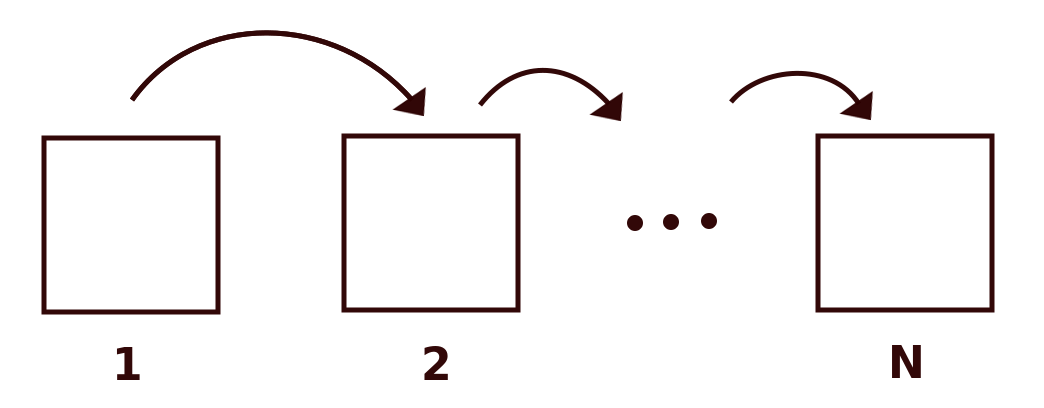
\includegraphics[width=0.8\textwidth]{images/framebuffers.png}
\end{figure}
If we have $N-1$ textures, and let $N$ represent the application window,
then for $1 \leq i \leq N - 1$ we can use the image data in texture $i$
to run a shader which writes to texture $i+1$. The final image in
texture $N$ is rendered to the screen.
\end{frame}


%
%
%
\begin{frame}
\frametitle{Framebuffer Example: Conway's Game of Life}
\end{frame}


%
%
%
\begin{frame}
\frametitle{Summary}
We have seen the texture coordinate system.

\vspace{5mm}
We have seen methods for texture sampling.

\vspace{5mm}
Some code examples have shown how textures can be used in OpenGL 3.3.
\end{frame}


%
%
%
\begin{frame}
\frametitle{References}
\nocite{*}
\bibliography{refs}{}
\bibliographystyle{alpha}
\end{frame}



\end{document}
